% Apêndices
\begin{apendicesenv}

\partapendices

\chapter{Discussões sobre a verticalização}
\label{appendix:verticalizacao}

Assumindo prédios como paralelepípedos, ou seja, todos os andares apresentam a mesma metragem, é possível traçar relações geométricas nas quais a área ocupada é a superfície que representa a base do paralelepípedo, o número de pavimentos sua altura e a área construída seu volume (Figura \ref{fig:desenho}). Nesse sentido, as relações apresentadas na Equação \ref{eq:pavimentos}, que apresenta diferentes formas de calcular a verticalização, ficam mais claras. Na equação, AC representa a área construída; AO, a área o cupada; AT, a área do terreno; CA o coeficiente de aproveitamento e tx\_ocupacao, o percentual da área do terreno que é ocupada. Usando o procedimento apresentado, em regiões que possuem o mesmo CA, quanto menor for a taxa de ocupação do terreno, maior será a verticalização. Analogamente, para dois lotes com a mesma ocupação de terreno, quanto maior for o CA, maior é a verticalização.

\begin{figure}[h]
    \centering
    \caption{Representação do prédio como um paralelepípedo}
    % 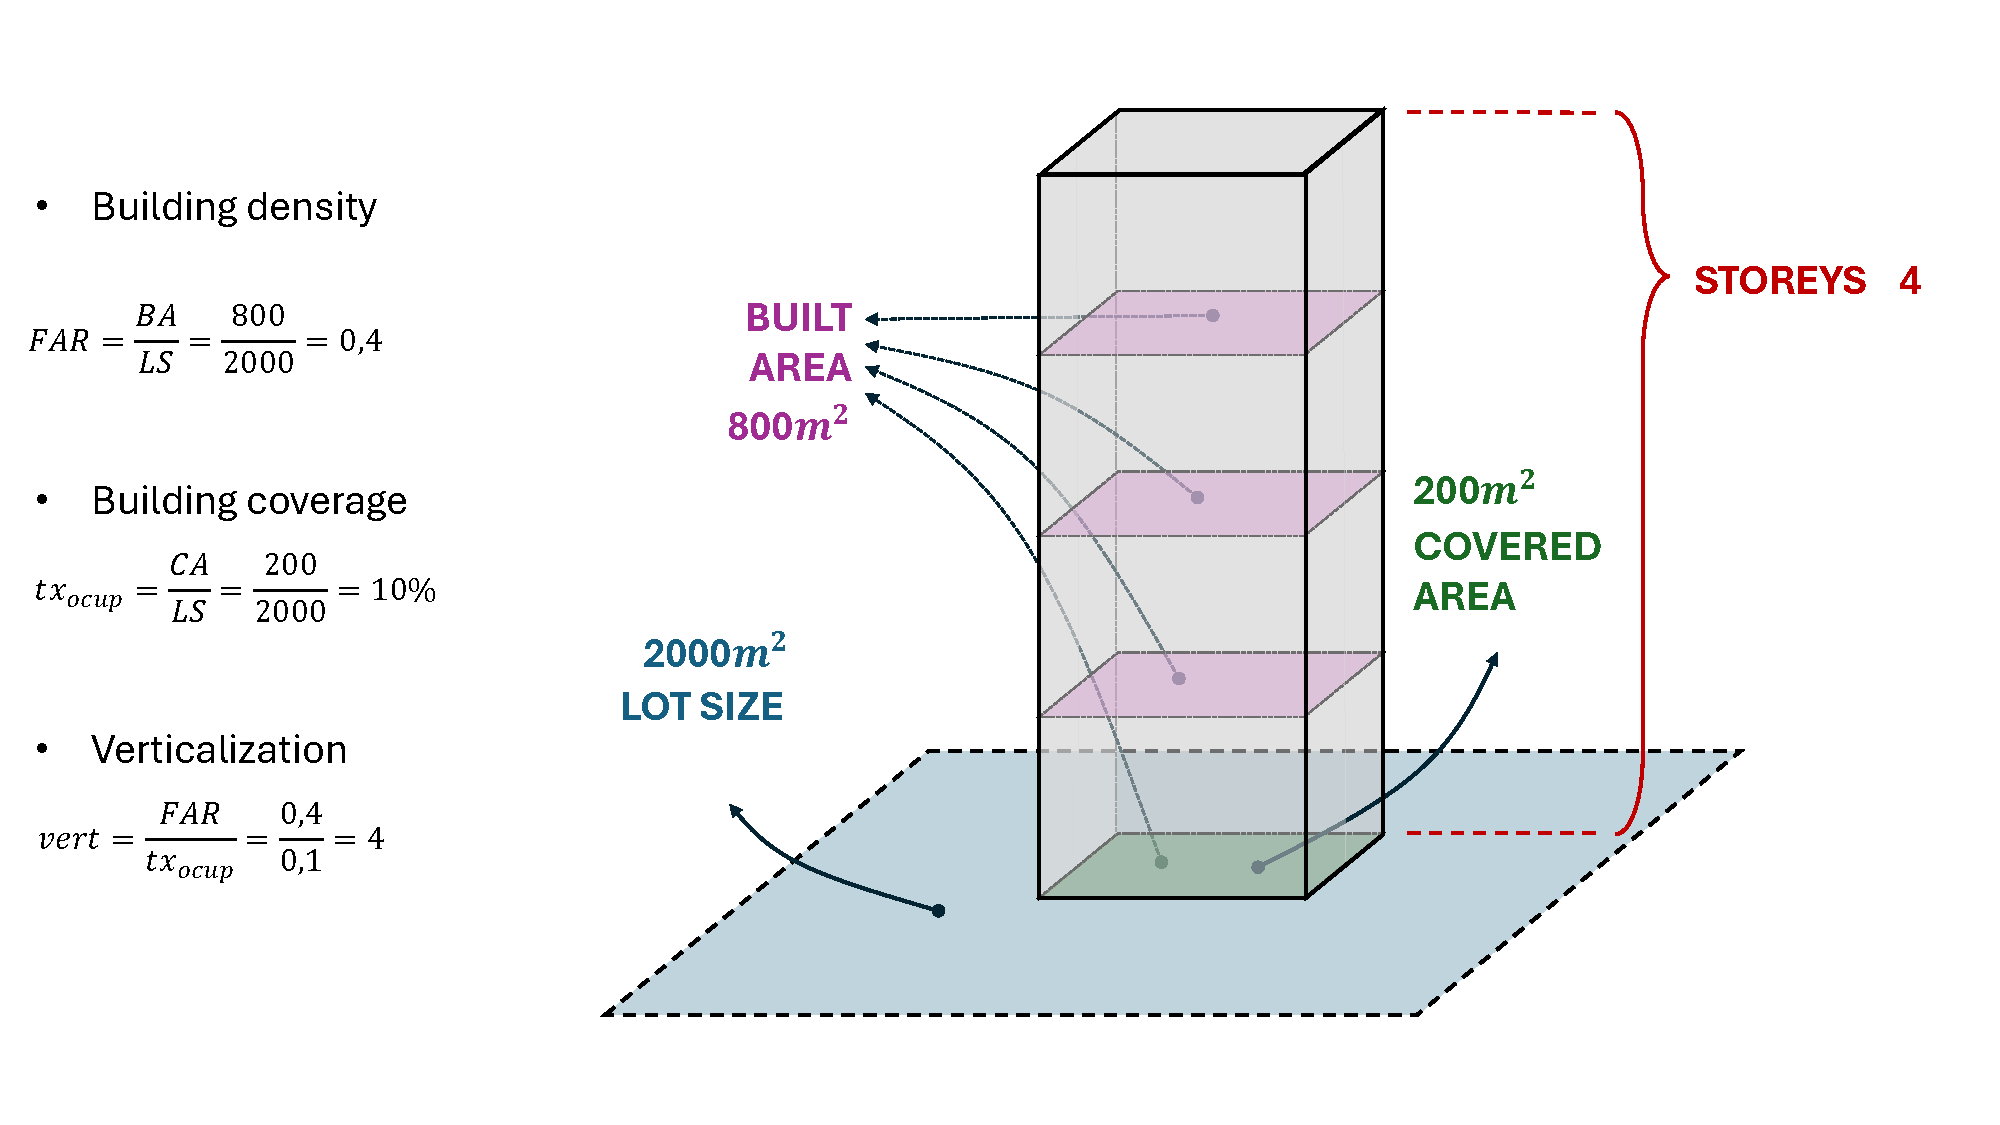
\includegraphics[width = \linewidth]{imagens/desenho.pdf}
    \label{fig:desenho}
\end{figure}

\begin{equation}
    \text{Pavimentos}=\frac{\text{AC}}{\text{AO}}=\frac{\text{AC}}{\text{AT}\cdot\underbrace{\frac{\text{AO}}{\text{AT}}}_\text{tx\_ocup}}=\frac{\text{AC}}{\text{AT}}\div\frac{\text{AO}}{\text{AT}}=\frac{\text{CA}}{\text{tx\_ocup}}
    \label{eq:pavimentos}
\end{equation}
    
Dessa forma, o número de pavimentos nunca será maior do que o CA, dado que a taxa de ocupação sempre é um número que varia entre zero e um. Na Figura \ref{fig:ca-vert} é possível observar a relação entre as duas variáveis. Para lotes muito pequenos, as duas medidas geralmente são iguais, visto que geralmente se ocupa 100\% da área do terreno. Na medida em que a verticalização aumenta, é observável que o CA não acompanha este crescimento, o que indica que há uma queda na taxa de ocupação.

\begin{figure}
    \centering
    \caption{Relação entre densidade construtiva e verticalização}
    % 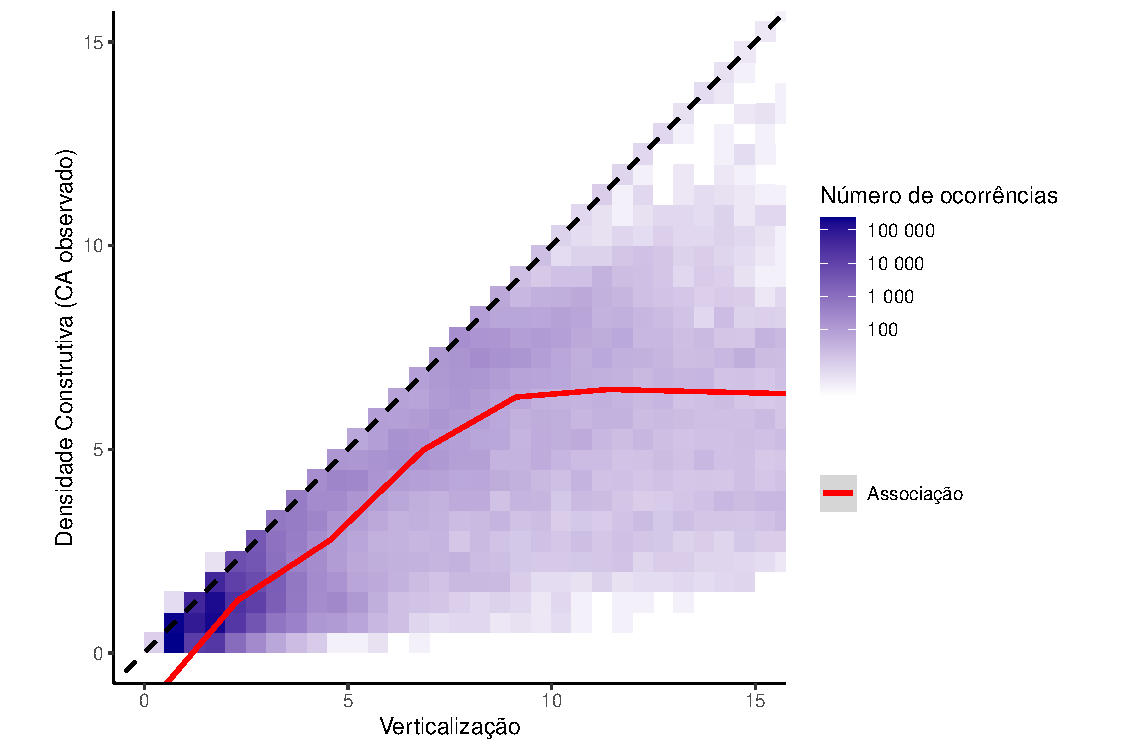
\includegraphics[width = \textwidth]{imagens/ca_vs_verticalizacao.pdf}
    \label{fig:ca-vert}
\end{figure}


\end{apendicesenv}
    
    